\documentclass[
	draft=true,
	paper=a4,
	fontsize=11pt,
	twoside=true,
	captions=tableheading,
]{scrreprt}
\usepackage[headsepline]{scrlayer-scrpage}
\pagestyle{scrheadings}
\automark[section]{chapter}

\usepackage[british, ngerman]{babel}

\usepackage{lipsum}

\usepackage[utf8]{inputenc}
\usepackage[T1]{fontenc}
\usepackage{microtype}
\usepackage{FiraSans}
\usepackage[lining]{FiraMono}
\usepackage[rm]{noto}

%\usepackage{float}
\usepackage{booktabs}
\usepackage{amsmath, amssymb}
\usepackage{csquotes}

\usepackage[colorlinks]{hyperref}

\setkomafont{captionlabel}{%
	\bfseries
}
\setcapindent{0em}

\usepackage[
	backend = biber, % Sets biber as backend.
	style = authoryear-icomp, % Use [author, year] citing with ibid. when duplicate.
	maxnames = 3, % Truncate lists above 3 entries (e.g. names). Both citing and bib.
	minnames = 3, % Truncate to 3 entries (e.g. names). Both citing and bib.
	backref = true,
	isbn=false,
]{biblatex}
\addbibresource{../references/references.bib}
\addbibresource{../references/websites.bib}
\addbibresource{../references/unpublished.bib}

\usepackage[nomain, nonumberlist, toc, acronym]{glossaries}
\loadglsentries{abkuerzungen.tex}
\makeglossaries

%\includeonly{titlepage, declaration_of_originality, thanks, abstract}

\begin{document}

\pagenumbering{roman}	
\begin{titlepage}
	\begin{center}
		\LARGE\textbf{\textsc{Universität Bremen}}\\
		\large\textbf{\textsc{Fachbereich 3: Mathematik/Informatik}}\\
		\vspace{2cm}
		\LARGE \textbf{\textsf{Arbeitstitel}} \\
		\vspace{2cm}
		\LARGE\textbf{\textsc{Masterarbeit}}\\
		\vspace{0.5cm}
		\large
		im Studiengang\\
		\enquote{Informatik Master of Science}\\
		\vspace{1cm}
		\normalsize
		vorgelegt am: \dots \\
		\vspace{3.5cm}
	\end{center}
	\vfill
	\hrule
	\vspace{1em}
	\normalsize{
		\begin{tabular}{ll}
			Name: & {Ralf Manuel Morawe} \\
			Matrikelnummer: & {2615732} \\
			Studiengang: & Informatik\\
			Fachsemester: & 4\\
			Erstgutachter: & {Prof. Dr. Johannes Schöning} \\
			Zweitgutachter: & {\dots} \\
		\end{tabular}\\
	}
\end{titlepage}
\cleardoublepage
\chapter*{Selbstständigkeitserklärung}
\thispagestyle{empty}

Hiermit erkläre ich, dass ich die vorliegende Arbeit selbstständig angefertigt, nicht anderweitig zu Prüfungszwecken vorgelegt und keine anderen als die angegebenen Hilfsmittel verwendet habe. Sämtliche wissentlich verwendete Textausschnitte, Zitate oder Inhalte anderer Verfasser wurden ausdrücklich als solche gekennzeichnet.\\[2ex]
Bremen, den \today\\[6ex]

\begin{tabular}{l}\toprule
	\centering\footnotesize Ralf~Manuel~Morawe
\end{tabular}
\cleardoublepage
%\chapter*{Danksagung}
\thispagestyle{empty}
\lipsum[10-11]
\cleardoublepage
%\chapter*{\abstractname}
\thispagestyle{empty}
\lipsum[1]

\cleardoublepage

\begin{otherlanguage}{british}
\chapter*{\abstractname}
\thispagestyle{empty}

\lipsum[2]

\end{otherlanguage}
\cleardoublepage

\tableofcontents
\printacronyms[title=Abkürzungsverzeichnis]
\cleardoublepage
\pagenumbering{arabic}

\chapter{Einleitung}
\label{chap:einleitung}

Durch den technischen Fortschritt in den letzten Jahren hat sich der Einsatz von \emph{Augmented Reality} (AR) und \emph{Virtual Reality} (VR) in verschiedenen Anwendungsbereichen etabliert \parencite{Krevelen2010, Zhao2009, Sharples2008, Jung2008}.
Als Nutzerschnittstelle dienen dienen in vielen Anwendungen Smartphones, da die Sensoren (Kameras, Gyrosensor etc.) nun ausreichen, um einfache AR-/VR-Inhalte zu präsentieren \parencite{Li2017b,Feng2017,Yoo2015,Mulloni2012}.
Neben Smartphones ermöglichen Head-Mounted Displays (HMDs) die Anzeige von \emph{Mixed-Reality-} (MR) und VR-Inhalten.
Beispielsweise sind hier die \emph{Microsoft HoloLens} \parencite{Microsoft2018} als AR-HMD oder die \emph{Oculus Rift} \parencite{Facebook2018} und \emph{HTC Vive} \parencite{HTCCorporation2018} als VR-HMD zu nennen (siehe \autoref{fig:devices}).
\begin{figure}[hb]
    \centering
    %\imagebox{%
    \begin{minipage}{0.3\textwidth}
        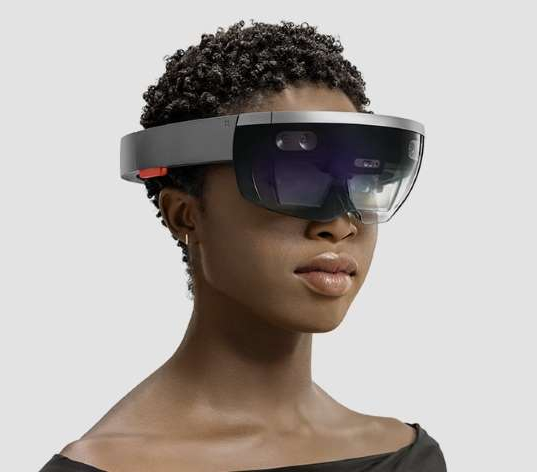
\includegraphics[width=.9\linewidth]{figures/Microsoft2018_HoloLens_worn}
    \end{minipage}%
    \hfill
    \begin{minipage}{0.45\textwidth}
        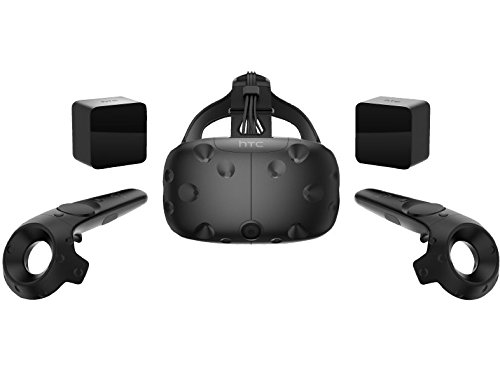
\includegraphics[width=.9\linewidth]{figures/htc_vive}
    \end{minipage}%
    \hfill
    \begin{minipage}{0.25\textwidth}
        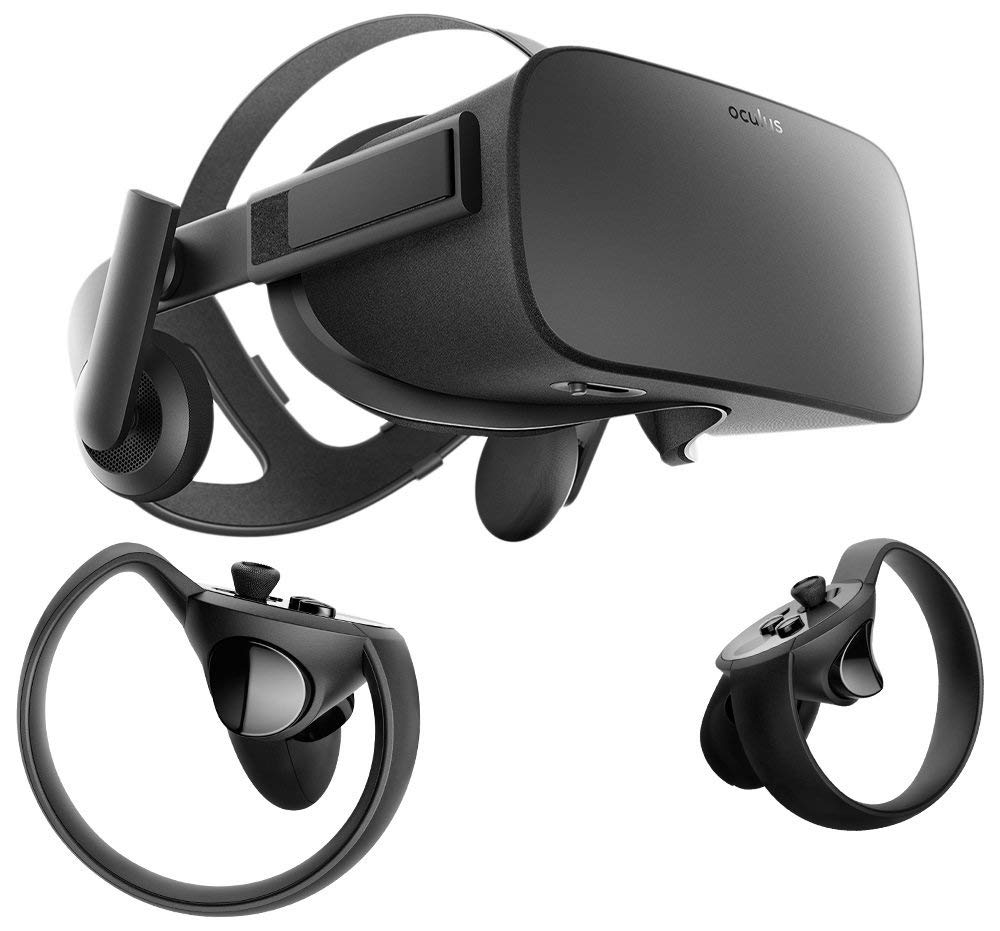
\includegraphics[width=.9\linewidth]{figures/oculus_rift}
    \end{minipage}%
    %}
    \caption{Diverse MR- und VR-HMDs. Microsoft HoloLens (Links), HTC Vive (Mitte) und Oculus Rift (Rechts). \quelle{\cite{Microsoft2018, Amazon2018b, Amazon2018}}}
    \label{fig:devices}
\end{figure}

Bei AR wird die Grenze zwischen dem Reellen und dem Virtuellen aufgehoben, indem virtuelle Inhalte in Echtzeit mit sechs Freiheitsgraden in die reale Welt überlagert werden.
\autoref{fig:mrtouch} zeigt z.B., wie virtuelle Nutzungsschnittstellen in die physische Welt platziert werden und über Berührungsinteraktion gesteuert werden können.
In der Vergangenheit wurde von Forschern AR unter anderem eingesetzt, um räumliche Informationen in der Umgebung von Nutzern anzuzeigen.
Beispielsweise wird die Navigation zwischen zwei Punkten augmentiert.
Die bisherigen Ansätze fokussieren die AR-unterstützte Schritt-für-Schritt-Navigation \parencite{Hoellerer1999, Hashish2017, Mulloni2012} und die Augmentierung von realem Kartenmaterial \parencite{Rohs2009, Morrison2009, Reitmayr2005}.
\begin{figure}[ht]
    \centering
    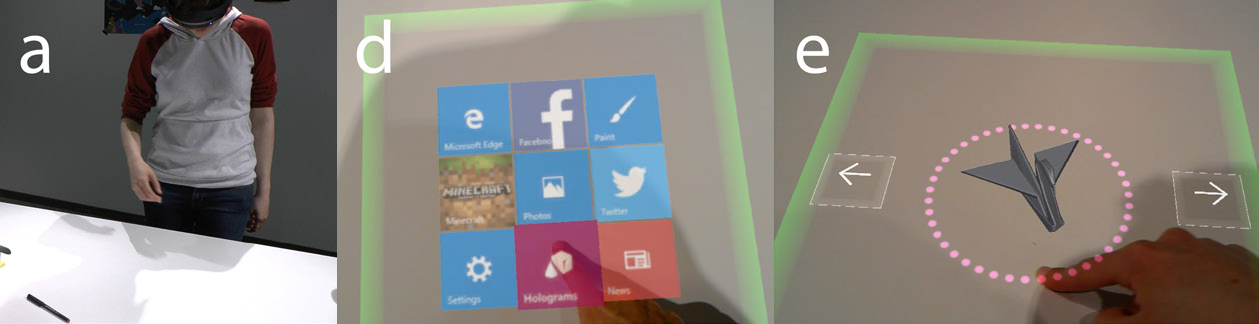
\includegraphics[width=\textwidth]{figures/mrtouch}
    \caption{Virtuelle Interfaces werden auf physischen Oberflächen platziert und mittels Berührungsgesten aktiviert. \quelle{\cite{Xiao2018}}}
    \label{fig:mrtouch}
\end{figure}

\section{Motivation und Ziel der Arbeit}
\label{sec:motivation_ziel}
Das Ziel \emph{dieser} Arbeit ist die Entwicklung einer neuartigen Form, räumliche Informationen mithilfe eines HMDs in eine AR-Szene zu integrieren: die \textbf{Megamap}.
Als Megamap wird in dieser Arbeit einer Kartendarstellung definiert, bei der ein dreidimensionales Abbild der Umgebung um den Nutzer herum gezeigt wird.
Die Karte ist in einem verkleinerten Maßstab zur Umgebung und ist in diese verankert.
Das bedeutet, wenn sich der Nutzer in der Welt bewegt, dann bewegt er sich auch auf der Karte.
Die virtuelle Karte verhält sich somit, als sei sie ein reales Objekt in der Umgebung.

Die ursprüngliche Idee für die Megamap-Darstellung stammt aus dem Spiel \emph{Tom Clancy's The Division} (TCTD) \parencite{Ubisoft2018} (siehe \autoref{fig:megamap}).
Eine Karte der Umgebung (eine Variante von New York) wird mit relevanten Spielobjekten und Ortsnamen \emph{im Spiel} als AR-Interface um den Charakter herum angezeigt.
Die Karte erlaubt dem Spieler unter anderem, Wegpunkte festzulegen (Navigation), interessante Punkte in der Umgebung anzuzeigen und zu filtern (Exploration) sowie die Ansicht durch Verschieben und Zoomen der Karte anzupassen.
Ebenso werden Missionsziele, andere Charaktere und Events durch Icons in der Karte hervorgehoben.
All diese Informationen sind vom aktuellen Kontext des Spiels abhängig.
Das heißt, es werden nur Informationen angezeigt die für die aktuelle Spielsituation des Spielers relevant sind.
\begin{figure}[t]
    \centering
    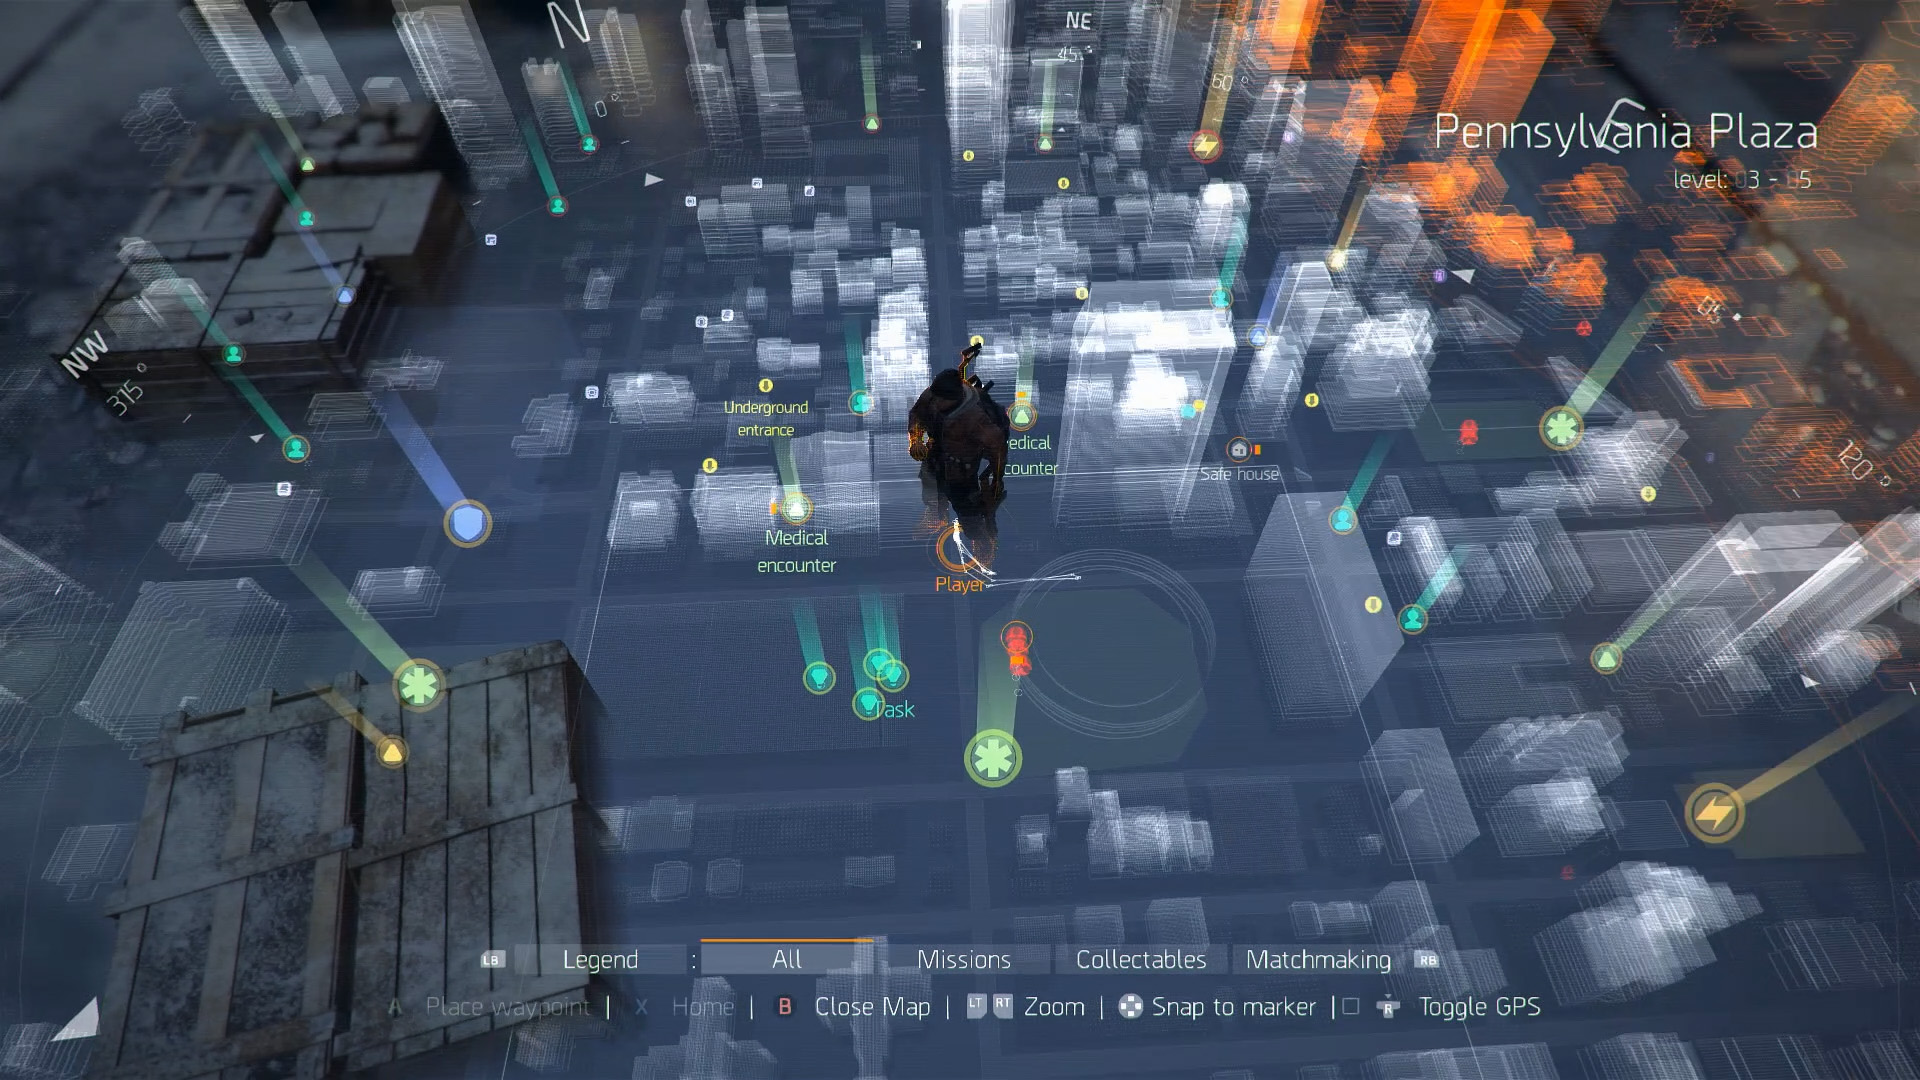
\includegraphics[width=\textwidth]{figures/the_division_megamap.jpg}
    \caption{Die \enquote{Megamap} aus \emph{Tom Clancy's The Division}. Symbole zeigen Missionsziele, Gegenstände und wichtige Orte im Spiel. \quelle{\cite{MYDIVISION.NET2014}}}
    \label{fig:megamap}
\end{figure}

%Eine Kartendarstellung existiert in dieser Form bisher nur im Spiel.
%In der realen Welt werden Karten zwar zunehmend durch AR/VR unterstützt.
%Eine Anwendung wie die Megamap aus TCTD, bei der die Karte in die Umgebung integriert ist, gibt es bisher aber noch nicht.
%Dafür gibt es mehrere Gründe:
%\begin{enumerate}
%    \item Die bisherigen Lösungen zur AR-unterstützten Kartenexploration stützen sich meistens auf die Überlagerung von virtuellen Information auf physische Objekte, beispielsweise eine reale Karte.
%    Dabei wird häufig ein Smartphone als \emph{Magic Lens} (\enquote{Magische Lupe},~\cite{Bier1994}) eingesetzt, auf dem die virtuellen Informationen vor dem Hintergrund der Kamera angezeigt werden.
%    Solch ein Ansatz ist jedoch nur Bedingt für den mobilen Einsatz geeignet.
%    Einem Fußgänger würde das gleichzeitige Halten einer Karte und eines Smartphones schwerfallen, besonders während des Laufens.
%    Auch der Einsatz eines Projektors, der die Informationen auf eine Karte projiziert, ist hierfür nicht geeignet.
%
%    \item Die durch virtuelle Helfer unterstützte Navigation ist ein Ansatz, der sich in der Forschung häufig finden lässt.
%    Allerdings ist die reine Navigation nicht der einzige Anwendungsfall in Bezug auf Kartenanwendungen.
%    Wie \textcite{Reichenbacher2001} detailliert beschreibt gibt es weitere Anwendungsfälle, die sich unter dem Oberbegriff der \emph{Kartenexploration} zusammenfassen lassen.
%    Darin eingeschlossen sind zum Beispiel die zuvor erwähnten Szenarios der Restaurantsuche oder der Anzeige von Fahrt- oder Öffnungszeiten.
%    Allgemein gesagt geht es bei der Kartenexploration um die \enquote{Entdeckung} von Orten anhand von Karten.
%    Diese Anwendungsfälle werden jedoch, in Bezug auf Unterstützung durch AR/VR, seltener behandelt als die Unterstützung der reinen Navigation.
%
%    \item Die Ansätze in der Literatur nutzen in der Regel Smartphones oder andere Handgeräte.
%    Obwohl die Entwicklung dieser Geräte technologisch rasch voranschreitet, sind sie auf die Möglichkeiten der Kamera-Bildsensoren, Gyrosensoren und GPS-Sensoren beschränkt.
%    Z.B. ist die dreidimensionale Rekonstruktion einer Szene, wenn überhaupt, nur sehr vereinfacht möglich.
%\end{enumerate}
%
%Die Integration der Karte in die Umgebung wäre jedoch von Vorteil.
%Denn eine von der Umgebung getrennte virtuelle Karte, wie es bei vielen aktuellen Smartphone-Anwendungen der Fall ist, kann die Aufmerksamkeit des Nutzers von der eigentlichen Umgebung ablenken.
%Die Nutzer müssen ständig das virtuelle Bild mit ihrer Umgebung abgleichen.
%Dies ist nicht nur ein zusätzlicher mentaler Aufwand.
%Im schlimmsten Fall kann es zu schweren Unfällen kommen wenn die Nutzer auf die virtuelle Darstellung achten oder die dargestellten Informationen beim Abgleich mit der Umgebung fehlinterpretieren \parencites{Medenica2011}{Lin2017}.
%
%Weitere Schwierigkeiten ergeben sich bei der Darstellung von \emph{Indoor}-Karten (Karten von Gebäuden).
%Die Überlagerung von mehreren Stockwerken stellt ebenso ein Problem dar wie die Tatsache, dass das GPS innerhalb von Gebäuden nicht verfügbar ist.
%Daher setzen sich viele existierende Ansätze mit der Navigation oder Lokalisierung innerhalb von Gebäuden auseinander.
%Der Anwendungsfall der Karten\emph{exploration} von Gebäuden wird hingegen bisher wenig behandelt.
%Weil kaum öffentliche Gebäudedaten verfügbar sind (im Gegensatz zu \emph{Outdoor}-Daten wie z.B. von \emph{Open Street Map} \parencite{OpenStreetMapFoundation2018}) wird die Situation weiter erschwert.

Eine Darstellung von räumlichen Informationen als Megamap bietet gegenüber herkömmlichen Ansätzen einige Vorteile:
\begin{itemize}
    \item Durch die Verwendung des HMDs bleiben die Hände der Nutzer frei. %
    Sie können die Karte nutzen und gleichzeitig mit beiden Händen mit der Umgebung interagieren.

    \item Da die Kartenansicht in die Umgebung der Nutzer integriert ist, müssen Nutzer die Kartendarstellung mit der Umgebung nicht wiederholt abgleichen. %
    So wird der Umgebung genug Aufmerksamkeit geschenkt und der mentale Aufwand der Nutzung wird verringert \parencite{Bark2014, Narzt2006, Kim2009}.

    \item Dadurch, dass die Karte in die Umgebung verankert ist und sich mit ihr mitbewegt, kann die Megamap auch während der Fortbewegung genutzt werden.

    \item Mit der Megamap können sowohl Außen- als auch Innenbereiche (z.B. Gebäude) dargestellt werden.
\end{itemize}

Die Recherche des Verfassers ergab keine Anwendungen, die das zuvor beschriebene Konzept einer Megamap umsetzen.
Daher wird im Rahmen dieser Arbeit eine Megamap-Anwendung entwickelt.
Spezifisch zielt die Anwendung auf die Nutzung in Innenbereichen wie Gebäude ab, da bisherige MR-HMDs Probleme mit der Verwendung im Freien aufweisen \parencite{Schroeder2017, Strange2018}.

Da sich außerdem die bisherigen Ansätze mit der Karten\emph{navigation} (\enquote{von A nach B}) beschäftigen, wird in dieser Masterarbeit der Anwendungsfall der Karten\emph{exploration} fokussiert.
Bei der Kartenexploration geht es um die Erkundung von Umgebungen anhand von kontextbasierten Ortsdaten.
Kontextbasierte Ortsdaten sind Daten, die von der aktuellen Situation abhängig sind, wie z.B. der aktuellen Position des Nutzers (\textquote{Wo ist das von mir aus nächste Restaurant?}/\textquote{Wieviele Spielplätze sind in meiner Nähe?}).
Ortsdaten können ebenso von der Zeit abhängen (\textquote{Welche Supermärkte in der Gegend sind geöffnet?}).
Übertragen auf die Innenbereichsnutzung stehen mit der Megamap verschiedene explorative Funktionen bereit, beispielsweise das Suchen nach den Büros von Personen oder den Standorten von öffentlichen Druckern.
Nutzer können sich mit der Megamap einen detaillierten Überblick über das Gebäude verschaffen, in dem sie sich befinden.

Als Zielplattform dient das Vive-HMD.
HMDs haben gegenüber Smartphones einige technische Vorteile.
Positionen und Orientierungen der Nutzer sind über Tracking präziser möglich.
MR-HMDs wie die HoloLens oder die \emph{Magic Leap One} \parencite[siehe \autoref{fig:magic_leap}]{MagicLeap2018} verwenden Infrarotkameras, um Strukturen der Umgebung virtuell in Echzeit zu rekonstruieren.
Die reale Umgebung bleibt dank des durchsichtigen Glases weiterhin sichtbar.
Zudem können die Hände für Gesteninteraktionen oder Kontroller verwendet werden anstatt das Display halten zu müssen.
\begin{figure}[tb]
    \centering
    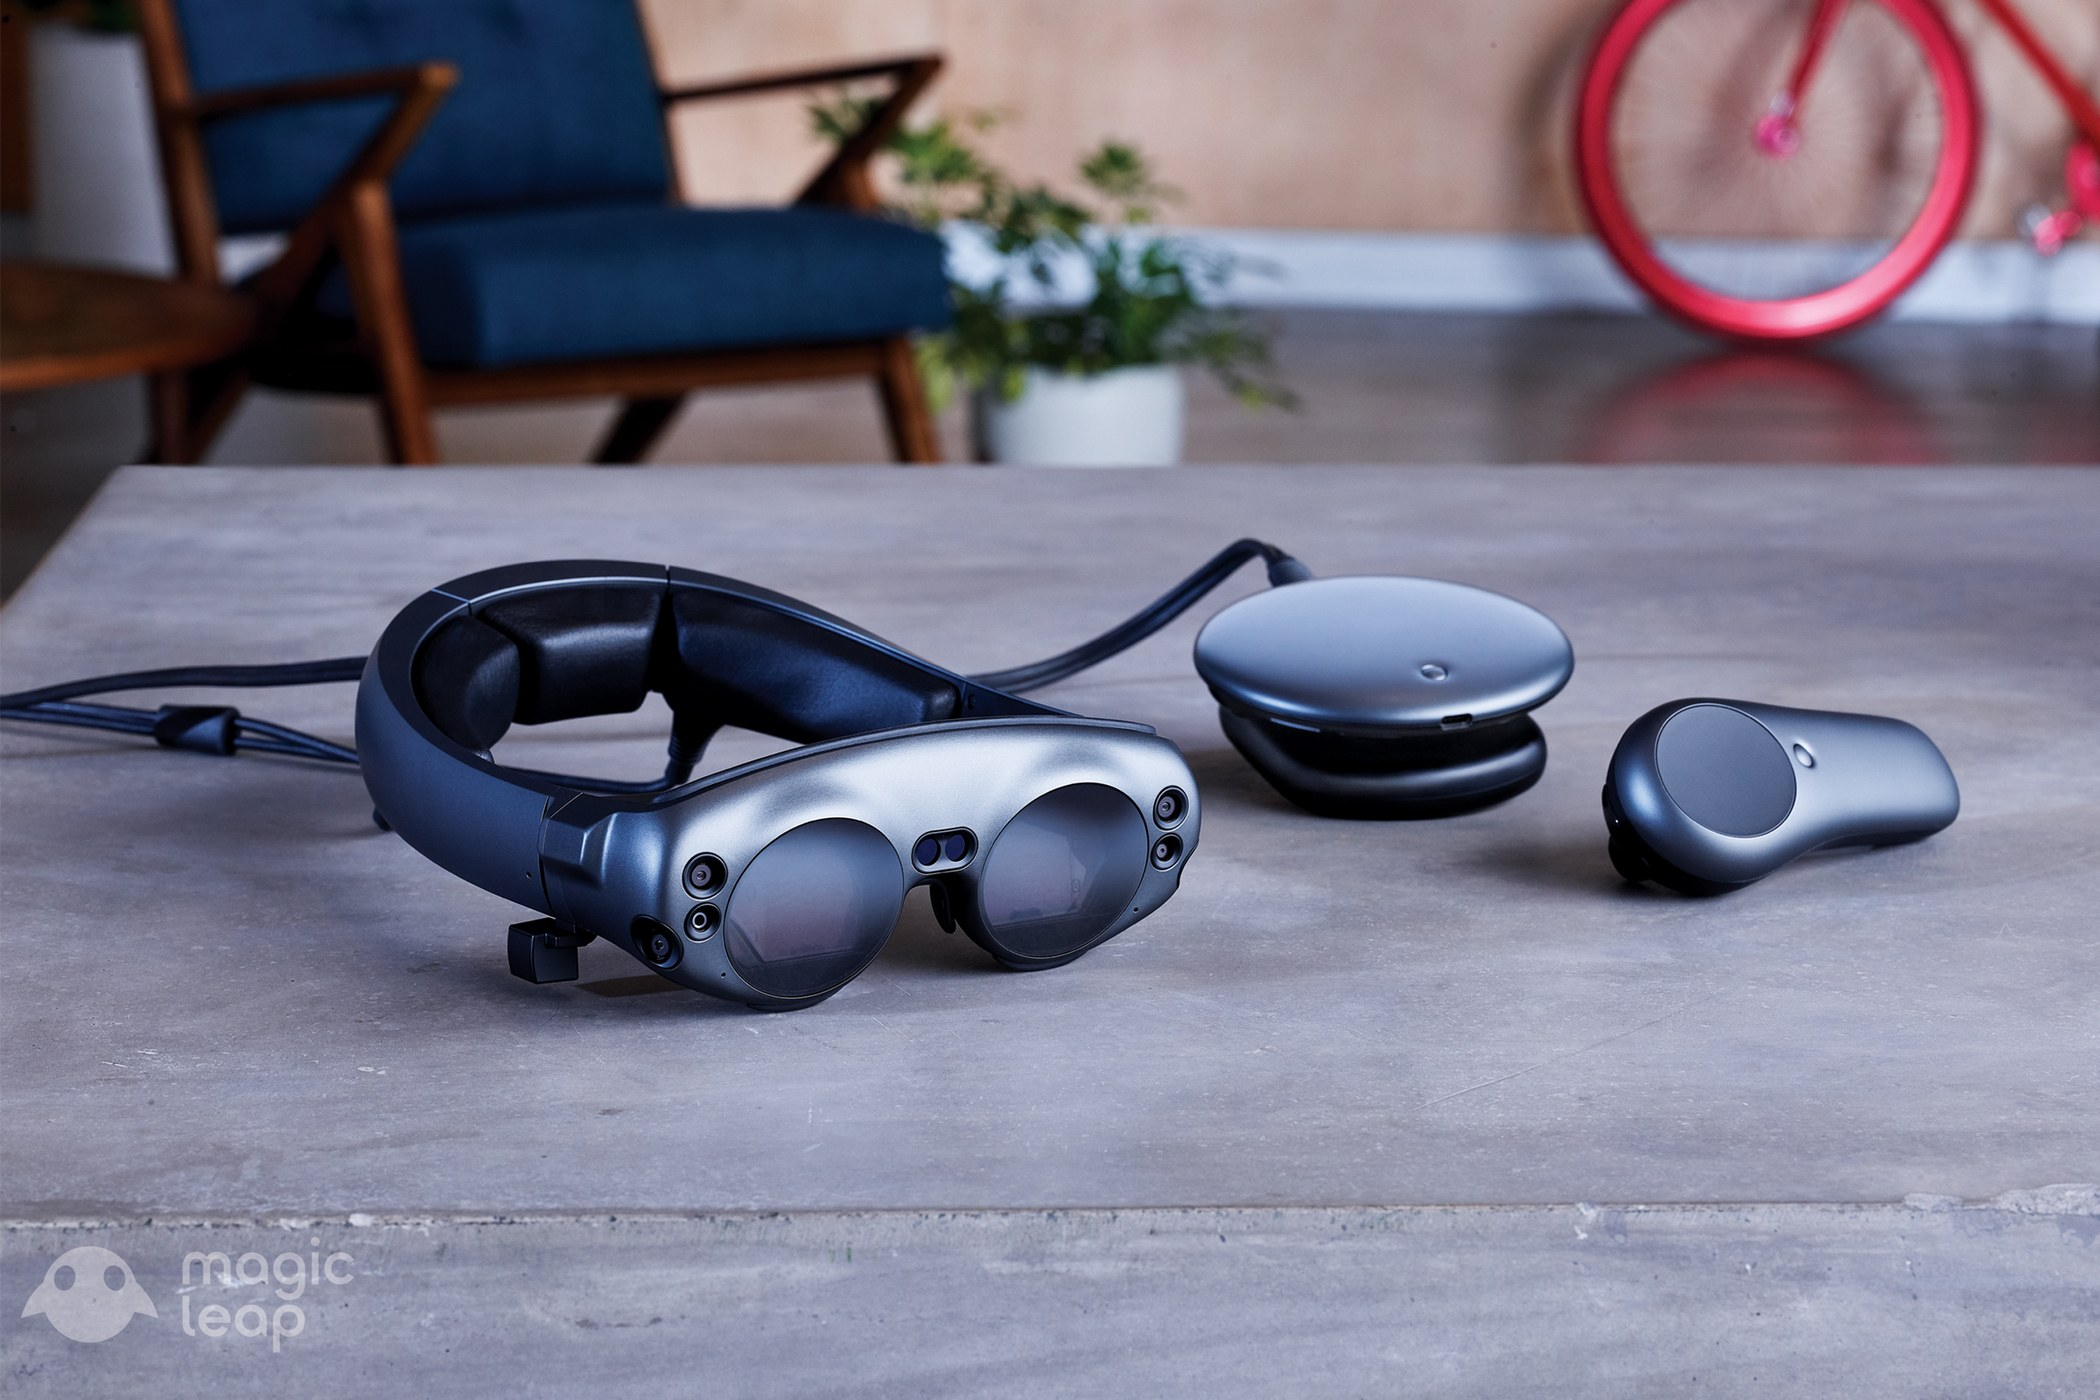
\includegraphics[trim={0, 7cm, 0, 7cm}, clip, width=\textwidth]{figures/magicleap}
    \caption{Das Magic Leap One MR-HMD. \quelle{\cite{MagicLeap2018b}}}
    \label{fig:magic_leap}
\end{figure}

Zu Beginn der Arbeit war das Ziel die Implementierung der Megamap für das Magic Leap One HMD.
Da dieses aber erst im späteren Verlauf der Arbeit veröffentlich wurde, wurde stattdessen die Implementierung für das Vive-HMD in VR umgesetzt.
Die \enquote{reale} Umgebung des Nutzers wird dabei virtuell nachgebildet.
Dadurch lässt sich die Megamap-Anwendung in zukünftigen Arbeiten auf ein MR-HMD übertragen.

%Die Implementierung der Megamap dient der Beantwortung der zentralen Fragestellung dieser Arbeit:
%\begin{quote}
%    \itshape
%    Ist eine in die Umgebung integrierte 3D-Megamap geeignet, um Nutzer bei der Exploration von Gebäuden zu unterstützen?
%\end{quote}
%Der Prototyp wird daher in einer Nutztungsevaluation getestet, um seine Effektivität für die Gebäudeexploration festzustellen.

%Als Inspirationsquelle für die Anwendung dienen neben bereits existierenden Kartenanwendungen wie Google Maps und Ansätzen aus der Forschung auch digitale Spiele.
%Da in Spielen Aufgaben wie Navigation und Exploration von großer Bedeutung sind, kann hier unterschiedliche Ansätze zur Navigations- und Explorationsunterstützung gefunden werden.
%Dies ist am Beispiel TCTD erkennbar.

Da die Idee für die Megamap einem Videospiel entspringt ist nicht unmittelbar klar, ob sich das Konzept auf die Nutzung in der realen Welt übertragen lässt.
Insbesondere, weil die Megamap aus TCTDs Dritte-Person-Perspektive (\emph{Third-Person Perspective}) in die Egoperspektive überführt wird.
Die Eignung der Megamap für die Kartenexploration wird daher am entwickelten Prototypen in einer Nutzerstudie überprüft.
Einerseits werden die subjektiven Eindrücke der Probanden von der Nutzung der Megamap festgehalten.
Andererseits wird die Performance im Vergleich zu einer herkömmlichen 2D-Darstellung einer Indoor-Karte verglichen.

\section{Struktur der Arbeit}
\label{sec:struktur}
Die restliche Arbeit ist in die folgenden Abschnitte unterteilt:

\noindent
Im nächsten Kapitel wird der Stand der Forschung und Technik zur Darstellung von dreidimensionalen Karten beleuchtet.
Die Unterschiede zum Konzept dieser Arbeit sowie deren Beitrag zum Thema werden ebenso herausgearbeitet.
\autoref{chap:concept} geht detailliert auf die Konzeptionierung der 3D-Megamap ein.
Es wird vor allem beschrieben, welche Interaktionen für die Kartenexploration wichtig sind und wie diese in der Megamap-Anwendung umgesetzt werden sollen.
Danach wird in \autoref{chap:implementation} die Implementierung der Anwendung beschrieben.
Ebenso werden Probleme bei der Implementierung erläutert, die für zukünftige Arbeiten beachtet werden sollten.
\autoref{chap:evaluation} präsentiert die Durchführung der Nutzungsevaluation der Anwendung sowie deren Ergebnisse.
Schließlich werden in \autoref{chap:closing} offene Fragen und Probleme dieser Arbeit genannt, welche für zukünftige Arbeiten von Interesse sind.
%
\cleardoublepage


\printbibliography[nottype=online]
\printbibliography[title={Online Referenzen}, type=online]

\end{document}
